\documentclass[tikz]{standalone}

\usepackage{tikz}
\usepackage{standalone}

\usepackage{siunitx}

\begin{document}
    \begin{tikzpicture}
        \node (nantes) at (0,0) {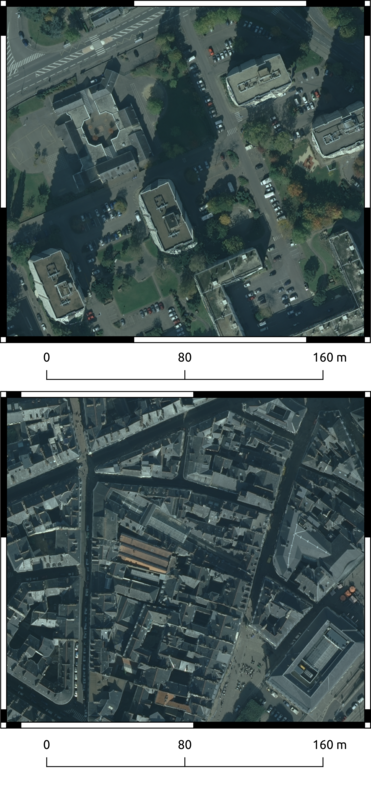
\includegraphics[height=10cm]{images/nantes}};
        \path (nantes.north) node[anchor=south, text width=4.5cm, align=center] (nantes_type) {\large Dense downtown w/. high towers.};
        \path (nantes.south) node (nantes_l) {\large (b) Nantes (748 buildings)};
        \path (nantes_l.south) node[anchor=north] {\large Img./DSM res.: \SI{10}{\cm}};
        \path (nantes.west) + (-4, 0) node (elancourt) {\includegraphics[height=10cm]{images/elancourt}};
        \path (elancourt.north) node[anchor=south, text width=4.5cm, align=center] (elancourt_type) {\large Industrial \& residential buildings.};
        \path (elancourt.south) node (elancourt_l) {\large (a) Elancourt (2009 buildings)};
        \path (elancourt_l.south) node[anchor=north] {\large Img./DSM res.: \SI{6}{\cm}};
        \path (nantes.east) + (4, 0) node (paris13) {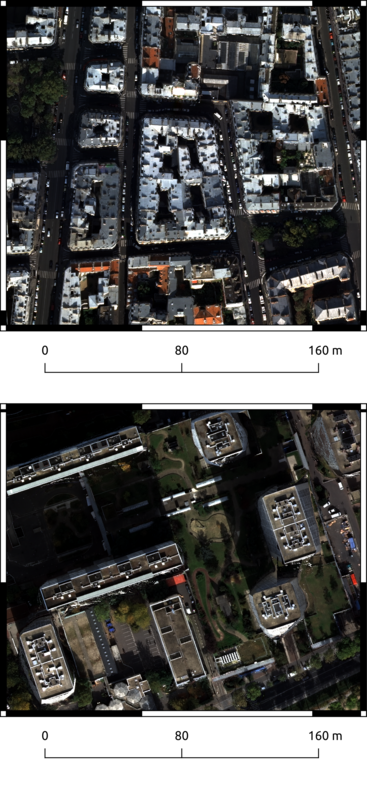
\includegraphics[height=10cm]{images/paris-13}};
        \path (paris13.north) node[anchor=south, text width=4.5cm, align=center] (paris13_type) {\large Hausmann style downtown w/. high towers.};
        \path (paris13.south) node (paris13_l) {\large (c) Paris-13 (478 buildings)};
        \path (paris13_l.south) node[anchor=north] {\large Img./DSM res.: \SI{10}{\cm}};
    \end{tikzpicture}
\end{document}